\documentclass{article}


\usepackage{arxiv}

\usepackage[utf8]{inputenc} % allow utf-8 input
\usepackage[T1]{fontenc}    % use 8-bit T1 fonts
\usepackage{hyperref}       % hyperlinks
\usepackage{url}            % simple URL typesetting
\usepackage{booktabs}       % professional-quality tables
\usepackage{amsfonts}       % blackboard math symbols
\usepackage{nicefrac}       % compact symbols for 1/2, etc.
\usepackage{microtype}      % microtypography
%\usepackage{lipsum}

\usepackage{graphicx}

\title{Paper title}


\author{
  Juliana Y.~Rhee\\
  Department of Molecular and Cellular Biology\\
  Center for Brain Science\\
  Harvard University\\
  Cambridge, MA 02138 \\
  \texttt{rhee@g.harvard.edu} \\
  %% examples of more authors
   \And
  Cesar Echavarria\\
  Department of Neuroscience\\
  Center for Brain Science\\
  Harvard University\\
  Cambridge, MA 02138 \\
  \texttt{email} \\
   \And
  Javier Masis\\
  Department of Molecular and Cellular Biology\\
  Center for Brain Science\\
  Harvard University\\
  Cambridge, MA 02138 \\
  \texttt{email} \\
  \And
 David D.~Cox \\
 Center for Brain Science\\
  Department of Molecular and Cellular Biology\\
  Harvard University\\
  Cambridge, MA 02138 \\
  \texttt{davidcox@g.harvard.edu} \\
  %% \AND
  %% Coauthor \\
  %% Affiliation \\
  %% Address \\
  %% \texttt{email} \\
  %% \And
  %% Coauthor \\
  %% Affiliation \\
  %% Address \\
  %% \texttt{email} \\
  %% \And
  %% Coauthor \\
  %% Affiliation \\
  %% Address \\
  %% \texttt{email} \\
}

\begin{document}
\graphicspath{./figures/}

\maketitle

\begin{abstract}
Preliminary paper outline with figures.
\end{abstract}


% keywords can be removed
% \keywords{First keyword \and Second keyword \and More}


\section{Introduction}
The brain's visual system translates ambiguous and rapidly-changing patterns of light falling on the retina into a coherent representation of the external world that can be used to guide behavior. The ability to recognize objects despite the enormous variation with which they can appear, \textit{e.g.}, due to viewing angle, scale, or lighting, is called invariant object recognition. The hierarchical organization of sensory cortex is thought to play a key role in its ability to extract and learn about latent structure from visual inputs. For example, visual object recognition in primates is thought to emerge through sequential processing across cortical areas in the ventral visual pathway~\cite{rustselectivity2010, DiCarlo:2007aa, dicarlo2012does, Chen2014682}, and numerous studies show increasing selectivity for complex stimuli at progressively higher levels of a sensory processing hierarchy~\cite{desimone1984stimulus, logothetis1996visual}.  However, the nature of the transformations that occur from one level of the hierarchy to the next remain poorly understood. 

Increasing evidence suggests rodents possess sophisticated visual machinery that would make them a tractable model for studying multi-level visual processing. Rats, in particular, can perform invariant object recognition tasks~\cite{cite, cite, cite}, and their visual cortex, namely, areas V1, LM, LI, and LL, exhibits properties similar to that of primates~\cite{cite, cite cite}. Here, we take advantage of optical methods, which allow simultaneous access to multiple brain regions with single-cell resolution, and present their first application to an animal model of invariant object recognition. We describe the macro- and micro-scale organization of V1, LM, and LI in the context of a range of stimulus classes. Specifically, we characterize feature tuning and object tuning in rat visual cortex to examine how neural circuits encode feature variations that either preserve object identity or alter object identity. 


\section{Retinotopic organization of rat visual cortex}
\label{sec:retinotopy}

\subsection{Optical mapping rat visual cortex}
See Figure \ref{fig:fig1}. Macroscale retinotopy is smooth across visual cortex. Visual field representation is non-uniform within visual areas. 

\begin{figure}[ht]
  %\centering
  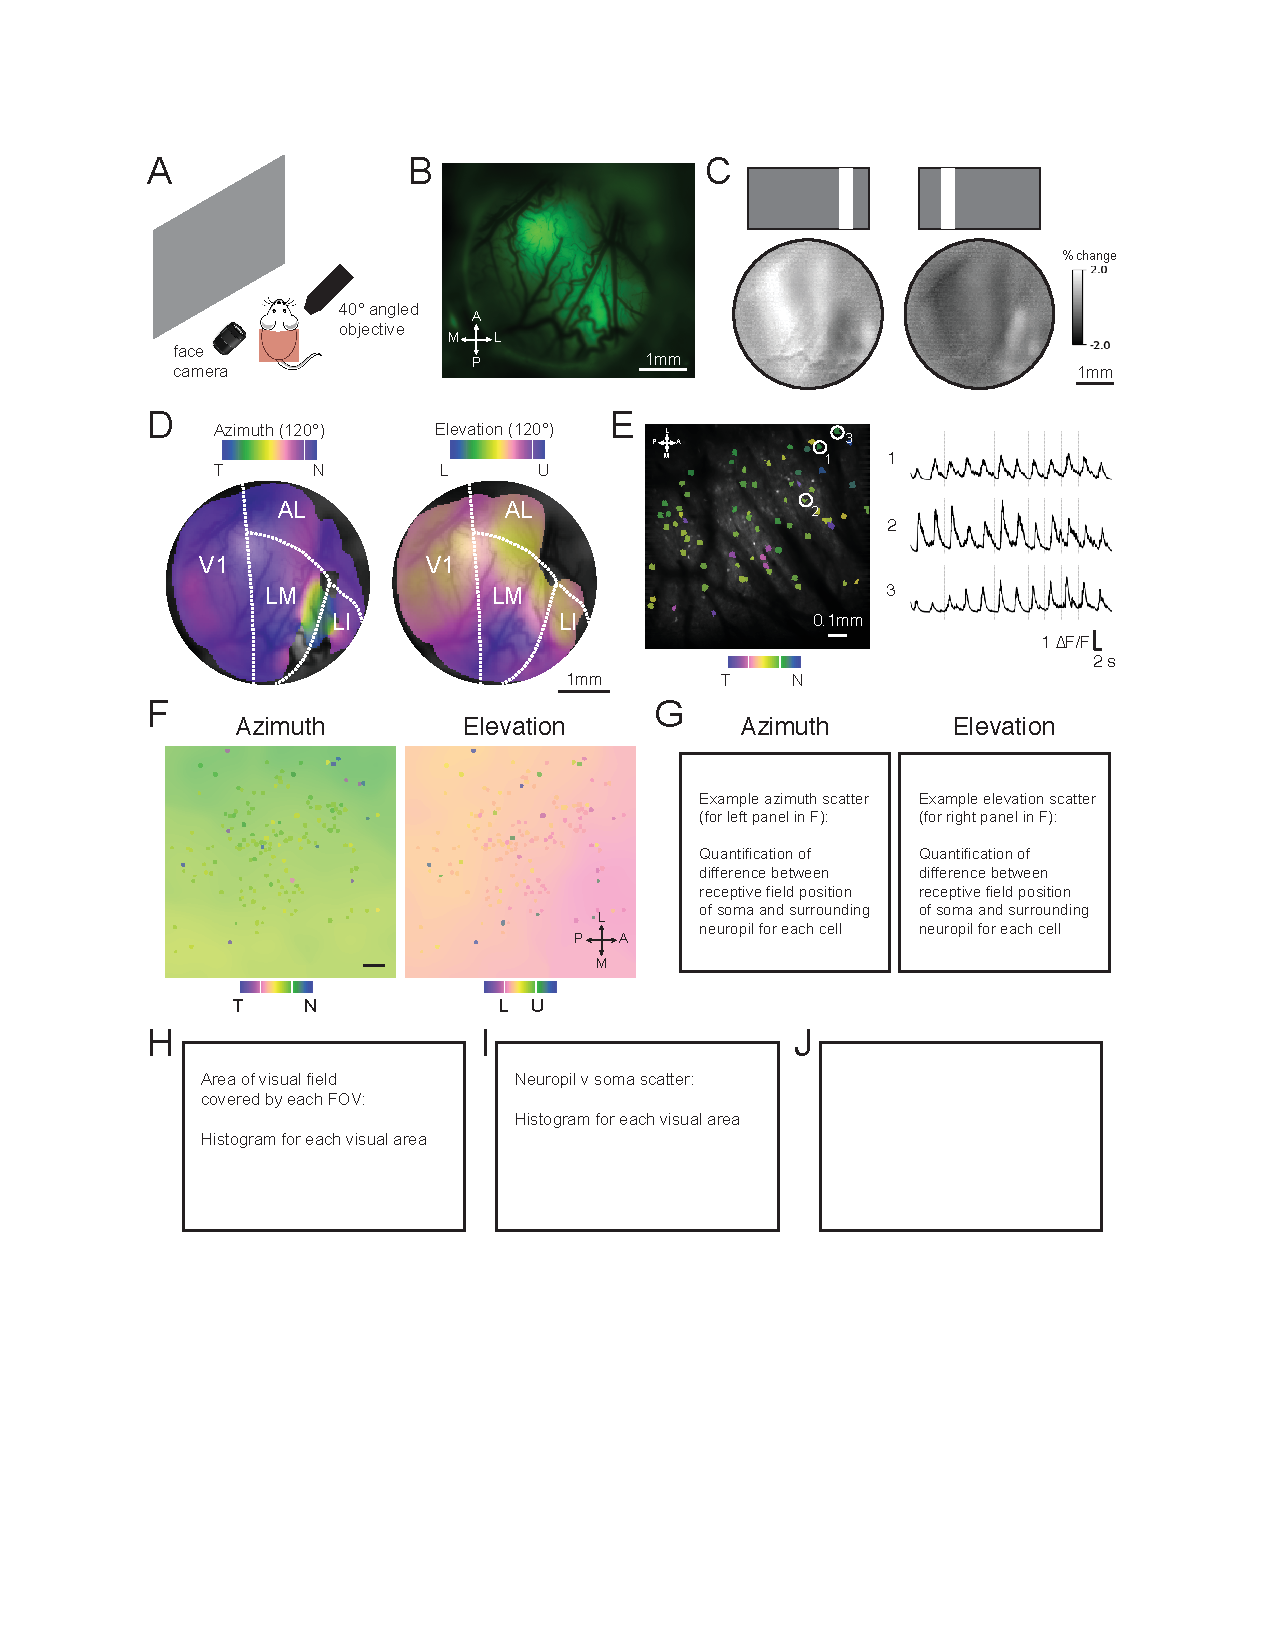
\includegraphics[width=\textwidth]{figures/retino.pdf}
  \caption{Macroscale retinotopy in rat visual cortex.}
  \medskip
  \small
  A.  Experiment setup.  
  B.  Epifluorescence image of an example cranial window with AAV9-GCaMP6f expression. Scale bar is 1mm.  
  C.  GCaMP6f response to a vertically-oriented moving bar. Average response to a 5 degree vertical bar (upper inset) on the nasal visual field (\textit{left}), and the temporal visual field (\textit{right}) in an example rat. 
  D.  Pseudo-colored maps of azimuth (\textit{left}) and elevation (\textit{right}) for the cranial window shown in C. V1 (primary visual cortex), LM (lateral-medial), LI (lateral-intermediate), AL (antero-lateral). N=nasal, T=temporal. 
  E.  Example of two-photon retinotopy. \textit{Left}: Average two-photon image of visually-evoked responses to a rightward moving bar stimulus, with cells color-coded by position. \textit{Right}:  Responses of the three cells circled on the left. Each trace represents the average of 4 repetitions of the rightward moving bar.
  F.  Maps of retinotopic preference for azimuth (\textit{right}) and elevation (\textit{left}).  Cells are color-coded by position. All other pixels contain a smoothed estimate of neuropil retinotopic preferences.
  G.  Difference in retinotopic preference between each cell and its surrounding neuropil along azimuth (\textit{left}) and elevation (\textit{right}) for the maps shown in F.
  H.  Area of visual field coverage for each two-photon FOV for visual areas V1, LM and LI. 
  I.  Degree of retinotopic scatter for all FOVs recorded in each visual area.
  J.  unknown
  \label{fig:fig1}
\end{figure}


\subsection{Receptive field properties in rat visual cortex}
See Figure \ref{fig:fig2}. Microscale retinotopy exhibits scatter. Rate of retinotopic change differs from V1 to Lm to Li. Slope of change reflects mirror reflections between visual areas. Receptive field sizes increase from V1 to Lm to Li. 

\begin{figure}[ht]
  %\centering
  \includegraphics[width=\textwidth]{figures/receptivefields.pdf}
  \caption{Microscale organization and receptive field properties of rat visual cortex.}
  \medskip
  \small
  A.  \textit{Left}:  Receptive field (RF) maps for three example cells in a V1 FOV. Blue traces, mean fluorescence signals for the stimulus at each of the stimulated locations. Color map, mean response 0-1s after stimulus onset.  \textit{Right}:  RFs estimated from 2d-Gaussian fits for all cells in the same FOV. 
  B.  \textit{Left}:  RF maps for three exmple cells in an LI FOV. Notation as in A. \textit{Right}:  RFs estimated from 2d-Gaussian fits for all cells in the same FOV.
  C.  RF centers as a function of cortical position along the azimuth axis relative to the FOV. Blue circles, RF centers fit to 10 repetitions at each position. Black, bootstrapped estimates of RF centers (vertical error bars, 95\% CI; horizontal markers, median of bootstrap distribution). Red, linear regression of RF center on cortical position (shaded area, 95\% CI).
  D.  Slope of linear regression of cortical position on RF position for V1, LM, and LI for azimuth (\textit{left}), elevation (\textit{middle}), and the average across azimuth and elevation conditions (\textit{right}) across all FOVs. Data points, measured slope for each FOV.  Boxes, inter-quartile (IQR) range for each visual area. Whiskers, 1.5*IQR.
  E.  Pairwise-distances in cortical space as a function of RF distance for V1, LM, and LI. Box plots as in D. 
  F.  Cumulative distribution of average RF sizes for V1, LM and LI. Average combines major and minor axes of fit RFs. 
  G.  Amount of RF overlap  and spread for cells in V1, LM and LI.  
  H.  Cumulative distribution of the correlation between cortical distance and stimulus condition for all pairs of neurons within each visual area. 

  \label{fig:fig2}
\end{figure}

\section{Feature tuning in rat visual cortex}
See Figure \ref{fig:fig3}. All visual areas exhibit axis selectivity, but LI cells show less axis selectivity. Direction selectivity is similar and low for all visual areas. Direction tuning is preserved across stimulus configurations if spatial frequency, size, and speed are varied. Tuning similarity is negatively correlated with spatial distance between cells for all visual areas, especially in LI. 

\begin{figure}[ht]
  %\centering
  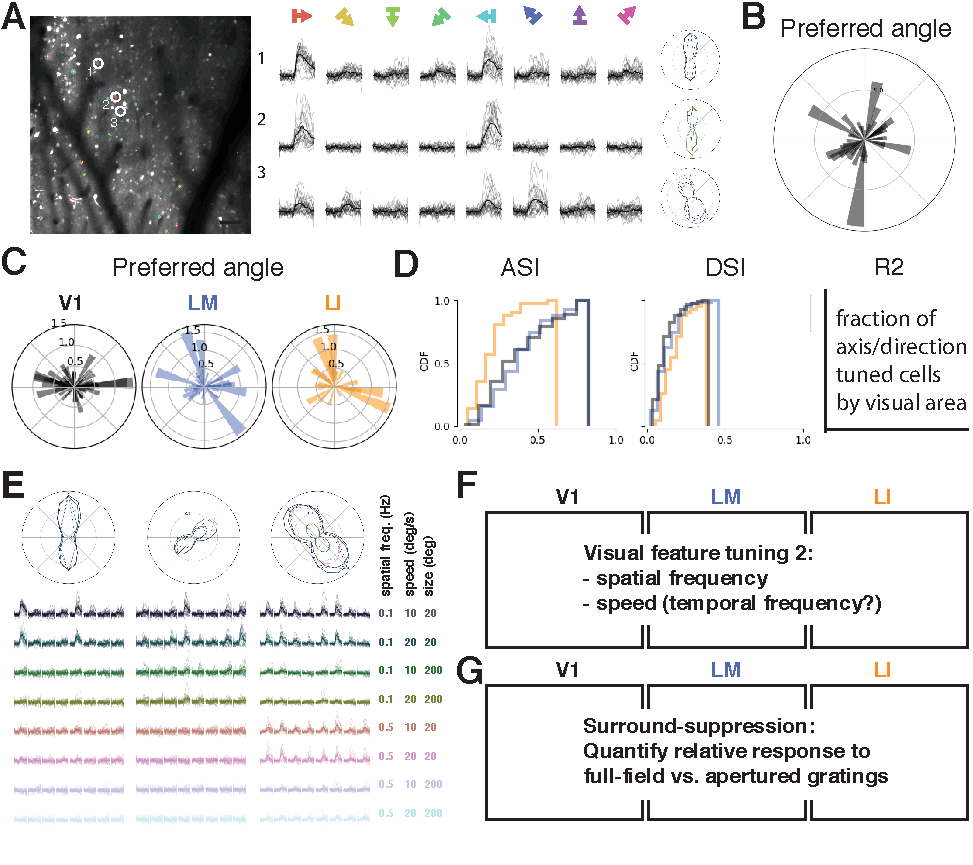
\includegraphics[width=\textwidth]{figures/features.pdf}
  \caption{Feature tuning.}
  \medskip
  \small
  A.  \textit{Left}:  Two-photon image of responses to drifting gratings, cells masked by preferred direction. \textit{Middle}: Responses of the three example cells circled on the left. Thin lines, trials; thicker lines, average. \textit{Right}:  Corresponding tuning curves for the responses on the left. 
  B.  Preferred directions for all tuned cells in the FOV shown in A.
  C.  Preferred directions for all tuned cells across FOVs by visual area.
  D.  \textit{Left}: Fraction of tuned cells out of all visual cells. Distributions of ASI (\textit{middle}) and DSI (\textit{right}).
  E.  Responses of three example cells to gratings across different stimulus configurations. \textit{Top}: Polar plots of raw (dotted lines) and fit (solid) tuning for the subset of conditions that passed fit criteria. \textit{Bottom}: Traces are trials for each grating direction, colors and rows denote the condition labeled at the right.
  F.  Spatial frequency and speed preferences by visual area.
  G.  Tuning modulation by stimulus size.
  H.  Tuning similarity as a function of cortical distance.
  I.  Distributions of correlations between cortical distance and stimulus condition for all pairs of neurons by visual area.
  J.  Average trial-to-trial correlations for pairs of responsive cells in a FOV, by visual area. Circles, upper triangle average of the correlation matrix for each FOV. Each point in this matrix is the correlation between two cells’ responses on all trials. 
  \label{fig:fig3}
\end{figure}


\section{Object preference in rat visual cortex}
See Figure \ref{fig:fig4}. Diversity of response profiles for object stimuli. Subsets of cells exhibit similar profiles of tuning (see panel B). All visual areas contain information about morph and size, which can be decoded with simple linear regression. Cells are more correlated in V1 than in LI. 

\begin{figure}[ht]
  %\centering
  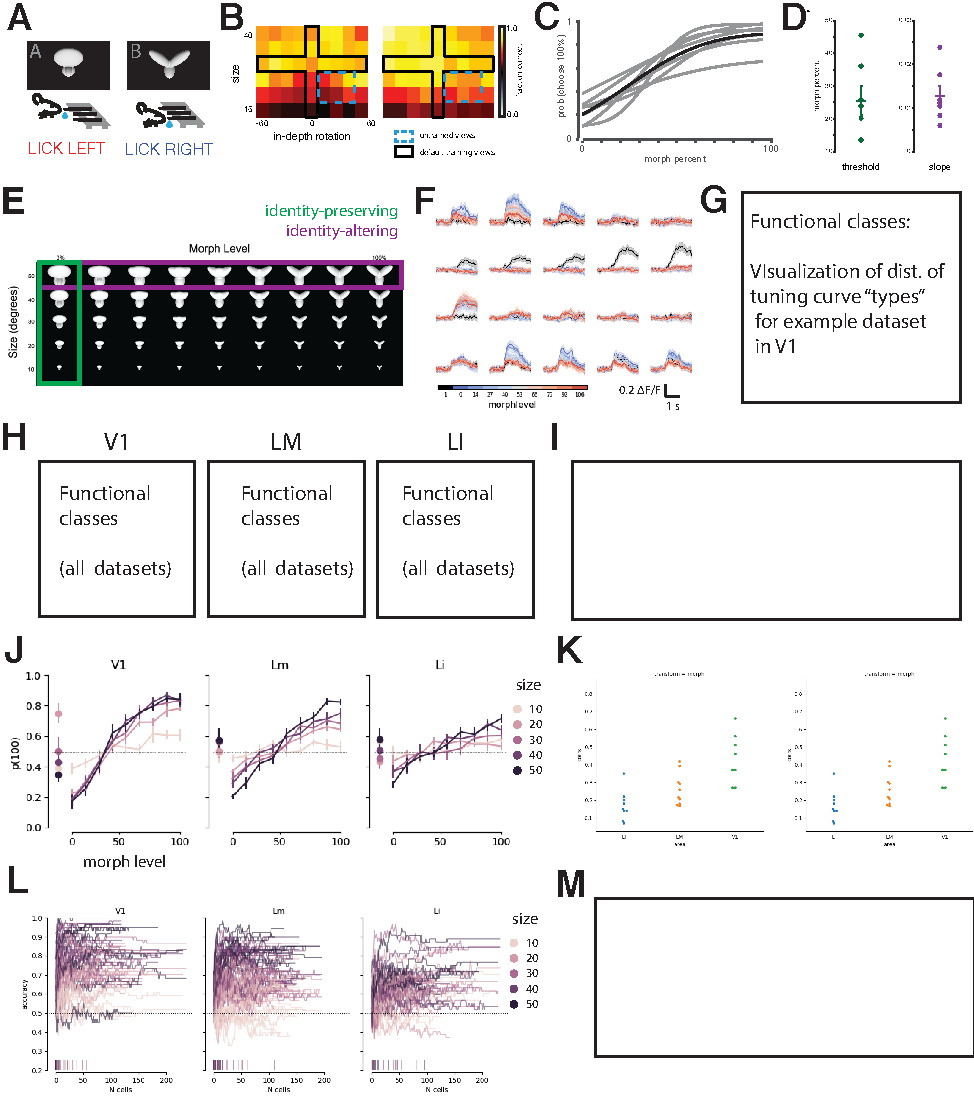
\includegraphics[width=\textwidth]{figures/objects.pdf}
  \caption{Object tuning.}
  \medskip
  \small
  A.  Schematic of stimulus conditions.
  B.  Responses of eight different cells.  Each row shows two examples of:  1)  Morph-tuned, size-tolerant, 2)  Luminance-tuned only, 3) Size-tuned only, 4)  Morph- and size/luminance-tuned. Traces show mean response (+/- sem) across repetitions for each stimulus condition.
  C.  Visualization of functional clusters for an example FOV.
  D.  Quantification of cluster distributions by visual area.
  E.  Linear relationship between neural responses and object features. \textit{Left}: Linear regression on size for an example FOV. Each point shows the predicted size versus the actual size of the stimulus presented on a trial. Blue gradient, morph level.  \textit{Middle}: Linear regression on morph. Notation as in the left. Blue gradient, size. \textit{Right}: Scatterplot of regression coefficients for morph and for size. Each data point is a cell. Lack of correlation suggests cells contribute differently to size and morph decoding.
  F.  Linear decoding of size and morph by visual area. Each data point is the correlation between the predicted and true values for one FOV, as shown in the scatterplots in the left and middle panels of E.  \textit{Left}:  Pearson’s correlation between predicted and true size.  \textit{Right}:  Pearson’s correlation between predicted and true morph level. 
  G.  Trial-to-trial correlations between pairs of visually responsive cells for one example FOV in each of V1, LM and Li. Each point in a matrix is the correlation between two cells’ response vectors, composed of the cell’s mean stimulus response for each trial.
  H.  Average of the upper triangle of the correlation matrix for each FOV, by visual area. Each data point is the average for one FOV. 
  \label{fig:fig4}
\end{figure}

\section{Models of object classification}
See Figure \ref{fig:fig5}. Rats trained to classify two objects can spontaneously generalize performance to novel, untrained identity-preserving transformations (vary size and in-depth rotation). Rats also spontaneously generalize performacne to novel, untrained identity-altering transformations in a predictable manner (as mesured by psychometric curves). To test whether naive neural responses of V1, Lm, and Li populations contain sufficient information to replicate the classification behavior in animals, we trained linear classifiers on the same task given to the behaving rats. Rats presented with object images learn to classify those images into 1 of 2 classes by  choosing one side to identify object A, and the other side to identify object B. Similarly, we trained linear SVMs with neural responses to these same object images to classify the responses as belonging to object A or object B. We then test the classifiers on intermediate morphs, which the classifiers have never before seen. Linear SVMs trained on neural data recorded from naive, passive-viewing rats are able to perform this task. V1 populations seem to best replicate the response profile seen in behaving rats, under the conditions tested. (More permutations of size/morph generalization must be done). 

\begin{figure}[ht]
  %\centering
  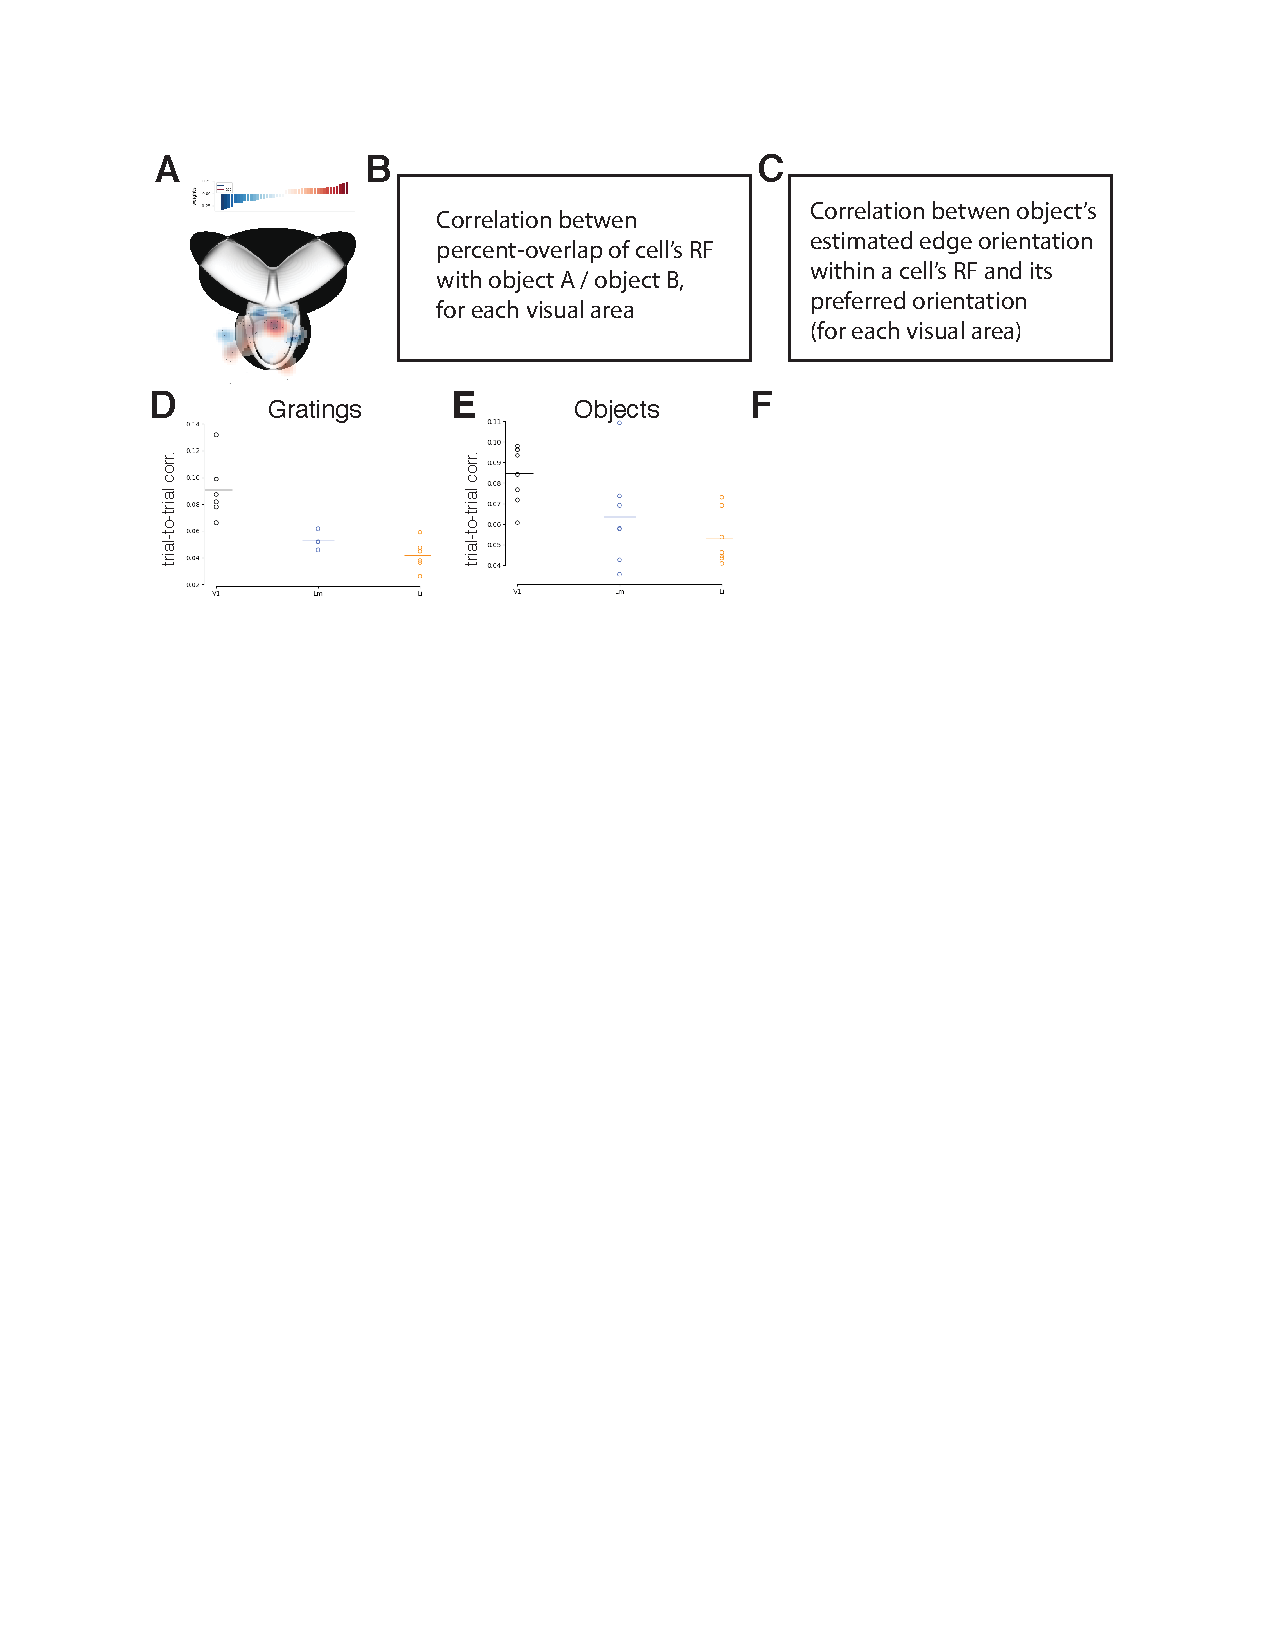
\includegraphics[width=\textwidth]{figures/allstim.pdf}
  \caption{Models for classification choices.}
  \medskip
  \small
  A.  Schematic of behavior paradigm.
  B.  Object classification in behaving rats.  Left and right panels show behavioral performance for two example rats.  Animals are first trained on the default views of the objects shown in A.  Black, additional trained views of the objects in A.  Blue, no-feedback trials to test generalization to untrained views. 
  C.  Psychometric curves for untrained classification of intermediate morphs that were parametrically varied between the objects in A. Gray, individual animals. Black, mean across animals. 
  D.  Threshold (\textit{left}) and slope (\textit{right}) of fit psychometric curves. Data points show values for each animal, bar shows mean across animals. 
  E.  Object classification by linear SVMs trained on neural data for each visual area.  N classifiers are trained on neural responses to objects A and B in a leave-one-out regime. Points at morph 0 and 100 show the average across FOVs of the average classification accuracy across folds. Points at intermediate morphs show the average choice across each presentation of a morph. Unconnected data points at the left show the average choice for size-matched luminance controls.  All classifiers trained and tested within a given size, denoted by color.  
  F.  Classification accuracy as a function of number of neurons for each visual area. Each line represents accuracy as a function of number of neurons for one FOV. As in E, all classifiers are trained and tested within a given size, denoted by color.  Vertical ticks on the x-axis show the number of neurons at 70\% accuracy, for each size, for each FOV.
  G.  Permutations of classifier training:  Size and morph generalization.
  H.  Difference image of object A and B, overlaid with density maps of classifier feature weights, positioned at the corresponding cell’s RF position and colored by its weight (inset shows weights sorted by strength).  Blue, object A. Red, object B.
  I.  Correlation between each cell’s preferred orientation and the estimated orientation of the subset of the object falling within its receptive field, for all cells in the example shown in H.
  J.  Simple model combining measured feature properties and object classification results for each visual area.
  \label{fig:fig5}
\end{figure}

\section{Methods}
\textbf{\textit{Headpost and cranial window implants}}

Headposts and cranial windows were implanted in naive rats (female Long Evans, 200-300g). Anesthetized with isofluorane in 100\% O2 (induction, 3-5\%; maintenance, 1.5-2\%) and placed on a heating pad (INFO) in a stereotaxic apparatus (INFO). Opthalmic ointment (Puralube) was applied to both eyes. For V1/Lm rats, heatposts were centered ~4.5-5 mm medial and 5-6 mm posterior to Bregma over the right hemisphere at 40 degrees. A 5-mm diameter craniotomy was performed at the center of the headpost, followed by a duratomy. Windows were stacks of seven 5 mm coverslips attached to one 5 or 7 mm coverslip, similar to~\cite{andermannsurgery, anotherone}. Coverslips were cured at least 24 hrs prior to surgery (UV-cured Norland Optical Adhesive 71).  Coverslip stacks were placed into the cranial window and sealed first with Vetbond (3M) followed by C&B Metabond (Parkell) to form a seal.  ...

\textbf{\textit{Viral injections}}

Injected 500nl of AAV9-GCaMP6f intracranially at 5-8 sites per rat. Mannitol and Fast-Green for spread and visualization during injections. Virus mixture injected at 20nl/min. Injection sites were 0.5-0.8mm apart. ...

\textbf{\textit{Epifluoresence imaging}}

Custom macrolens scope~\cite{GrinwaldMacro}. To identify the visual areas accessible in each window, we used epifluorescence calcium imaging to measure changes in responses to moving bar stimuli in lightly anesthetized mice. Include anesthesia details... A blue LED light source (LED info, Thor Labs) was used for excitation, and the green fluorescence was passed through a [filter info] emission filter and collected using [camera info].  Images (img size) were recorded using custom software (Python) at 25 Hz.

\textbf{\textit{Two-photon imaging}}

Lots to add here. Custom two-photon microscope, objective information and zoom, laser info, ...
FOV size and depths... Images were colleced at 44.65 frams/s, xx pixels/frame, using ScanImage (Matlab). 
Duration and structure of sessions, etc.

\subsection{Visual stimulation}

\textbf{\textit{Setup and stimuli}}

Monitor info...

To measure visual field coverage of each FOV, we presented a moving bar (2 degree width) at each cardinal direction~\cite{kalatsky2009}. To preserve the speed of the bar between azimuth and elevation conditions, the bar traversed the full extent of the monitor's width centered along the monitor's vertical extend (bar started and ended off screen). 12 cycles per trial, 3-4 trials per condition, 12-16 trials total. Bar presented at 0.13 or 0.24 cyc/s.

To estimate receptive field size and positions, we adapted a standard retinotopic mapping protocol~\cite{petreanuRF}. The screen was tiled into either 21x11 positions of 5 degrees or 11x6 positions of 10 degrees (see Suppl. Figure X). Drifting gratings (spatial frequency 0.25 Hz, speed 10 deg/s) were presented in square apertures of 5 degrees at each position, and pseudo-randomly switched between the 4 cardinal directions every 125 ms during the 500 ms stimulus presentation window. Each position was repeated 10 to 20 times. 

To measure visual feature tuning, we presented drifting gratings at 8 directions (0 to 315 degrees, steps of 45 degrees). Gratings were presented at either full screen or apertured, with the aperture size determined by the average receptive field size of the population recorded in previous  mapping sessions.  All directions were also presented at two spatial frequencies (0.5 and 0.1 Hz) to target the low and high end of known visual acuity levels~\cit{stuff}, and at two speeds (10 deg/s and 20 deg/s). This set of stimulus configurations resulted in 64 unique grating stimuli, which were repeated ~20 times in pseuedo-random order.

Objects. Behavior experiments, for current and previous paper~\cite{Zoccolan2009rats}. Morph stimuli were parametrically varied between the two anchor, default views of objects A and B using [details] (POVray). Each morph (7 intermediate morphs, plus 2 anchors) was presented at 5 different sizes (10-50 degrees, in 10 degree steps). For each size, mean luminance was measured with a photometer (INFO) to determine the levels needed to create full-screen controls matched for each size and object (see Suppl. Fig. X). This resulted in 50 unique object conditions, presented across ~30 repetitions each.

\subsection{Behavior experiments}
\textbf{\textit{Training}}

Three port task, train on default views of A and B~\cite{Zoccolan2009}. Test generalization to novel views and intermediate morphs. 

\textbf{\textit{Behavior analysis}}

Measuring performance within and across sessions, aggregate of animals. Compare multiple cohorts.
Psychometric curve fitting, etc.

\subsection{Image data processing}
\textbf{\textit{Image processing}}

Methods for motion correction, etc.

\textbf{\textit{Cell body mask identification}}

Methods for ROI selection (manual or CaImAn).

\textbf{\textit{Time course extraction and correction}}

Filtering and processing. Neuropil correction.

\subsection{Estimating retinotopic preferences}. 

\textbf{\textit{Widefield retinotopic maps}}

FFT analysis plus thresholding. Maps were smoothed (details) and filtered for visualization. Areal boundaries were delineated based on mirror reversals and etc...

\textbf{\textit{Estimating retinotopic preferences of cell bodies in two-photon}}

FFT analysis and filtering.


\textbf{\textit{Estimating retinotopic preferences of surrounding neuropil}}

FFT analysis and filtering/smoothing.

\textbf{\textit{Receptive field estimation}}

Two-dimensional Gaussian fits.  Bootstrap analysis. 
Threshold for cutoff was R2>=0.50.

\textbf{\textit{Retinotopic scatter}}

Bootstrap analysis, etc.


\subsection{Estimating tuning preferences in cells}

\textbf{\textit{Estimation of cells with significant visual responses}}

(Multiple methods so far, describing current):  For each cell and each stimulus condition, we determined the evoked response to be significantly different from noise if the amplitude of dF/F during the stimulus period exceeded 2.5 standard deviations above or below the mean baseline activity (computed using 0.5s or 1s prior to stimulus onset) for at least 10 out of the 44 time points (44.65 Hz frame rate * (0.5 s stimulus presentation + 0.5 s after stimulus offset).

To determine if a given cell showed a significant response at a particular stimulus configuration (size, speed, spatial frequency), we required that at least 2 out of the 8 directions at this given stimulus configuration evoked responses according to the above criteria. 

\textbf{\textit{Direction tuning curve fits}}

Direction tuning curves were estimated for each cell showing a significant response at a given stimulus configuration. 

Tuning curves were fitted with a two-peaked Gaussian with offset~\cite{somanypaper, alotofthem}:
EQUATION HERE
where R)(theta was the dF/F response for stimulus direction theta, etc.

First, in addition to the 8 tested points, a ninth point at 360 degrees was added, which was equal to the one at 0 degrees. The number of input points was increased from 9 to 25 by linear interpolation of the 9-point tuning curve. 

A bootstrap method was used to fit and estimate the tuning curve.  For each of 1000 iterations, the tuning curve was first computed by randomly sampling (with replacement) and averaging responses from 20 trials sampled from each of the 8 directions (to match the standard 20 repetitions in the actual experimental protocol). These 8-point tuning curves were interpolated, extended, then fit, as described above. The mean across the 10000 iterations were used as the final estimates of fitted parameters. 

To determine the quality of fits yielded by the above procedure, a combination of criteria was used [Liang, Cell 2018]~\cite{Liang2018cell}. For each iteration of the fitting procedure, a coefficient of determination, \textit{r}\textsuperscript{2}, was defined as the explained variance using least-squares regression to fit the data. Next, a combined coefficient of determination, \textit{r}\textsuperscript{2}\textsubscript{comb}, was computed by comparing the original tuning curve with the curve fit from the average of each fitting parameter across the 1000 iterations. A goodness-of-fit, \textit{G}\textit{\textsubscript{fit}}, was calculated as:

\textit{G}\textit{\textsubscript{fit}} = \bar{\sqrt{r\textsuperscript{2}}} (1 - IQR) \sqrt{r\textsuperscript{2}\textsubscript{comb}}

where IQR is the inter-quartile range (the difference between the 75\textsuperscript{th}- and 25\textsuperscript{th}-percentiles of $\surd$\textit{r}\textsuperscript{2}}  values across 1000 iterations). A cell was considered to have a well-fit tuning curve if the goodness-of-fit was greater than 0.60.  (more info on this).  The fitting procedure was performed separately for all stimulus configurations for which a cell was visually responsive, and the configuration yielding the maximum response was used.

\textbf{\textit{Axis and direction selectivity}}

Include axis-tuning and axis selective index (ASI) and direction selective index (DSI) calculations and equations. Bootstrap analysis, goodness-of-fit.

\textbf{\textit{Preferred direction of motion and preferred axis of motion}}

Bootstrap analysis, goodness-of-fit.

\textbf{\textit{Preferred spatial frequency}}

Bootstrap analysis, goodness-of-fit.

\textbf{\textit{Effect of surround suppression}}

Bootstrap analysis, goodness-of-fit.


\textbf{\textit{Functional clustering of object responses}}

Undetermined.

\subsection{Linear classification}
\textbf{\textit{Default view classification}}

Linear support vector machines, training/validating regime. Test samples, etc. Morph testing.

\textbf{\textit{Generalization across transformations}}
Details here.

\textbf{\textit{Training regimes}}
Details here.

\subsection{Simple model of object classification}
Unknown


\section{Supplementary Figures}


\subsection{Table of data}
Objects:  Cell counts reflect the number of visually responsive cells out of all manually selected ROIs.

Receptive fields:  Cell counts reflect the number of cells with successful receptive field fits (R2 >= 0.5) out of all manually selected ROIs.  

Gratings:  Cell counts reflect the number of cells with successfully fit tuning curves (see methods) out of all manually selected ROIs determined to be visually responsive.

(Met minimum requirement of N=3 rats per visual area for full battery of stimuli, with double this number for V1 and LM. Next steps:  Add 1-2 rats for V1 and LM. Add +3 rats for LI). See Table~\ref{tab:table}. 

\begin{table}[h]
 \caption{Data Summary}
  \centering
  \begin{tabular}{lllll}
    \toprule
    Experiment & Area & Rats & FOVs & Cells \\
    \midrule
    RFs & V1  & 5 & 12 & 1277     \\
        & LM  & 6 & 14 & 530      \\
        & LI  & 4 & 9 & 502      \\
    \midrule
    Gratings & V1  & 4 & 5 & 23     \\
             & LM  & 5 & 5 & 30      \\
             & LI  & 3 & 6 & 16      \\
    \midrule
    Objects  & V1  & 5 & 8 & 1493     \\
             & LM  & 5 & 7 & 1035      \\
             & LI  & 4 & 7 & 890      \\
    \bottomrule
  \end{tabular}
  \label{tab:table}
\end{table}

\subsection{General}
\begin{itemize}
\item Awake versus anesthetized recordings for receptive fields and gratings.
\item Face tracking analysis
\item Luminance measures for size-matched controls in objects experiment.
\end{itemize}

\subsection{Related to Figure \ref{fig:fig1}}
\begin{itemize}
\item Comparison of results across different thresholds for responsive cells for moving bar retinotopy.
\item Widefield azimuth and elevation maps (delineated) for all animals used in study.
\item Proportion of visual area image with two-photon across rats (visual field representation by visual area).
\end{itemize}
\subsection{Related to Figure \ref{fig:fig2}}
\begin{itemize}
\item Comparison of 5-degree versus 10-degree position tiling for V1 examples and LI examples.
\item Difference in rate of change between azimuth and elevation conditions for each visual area.
\item Quantification of retinotopic "scatter" or deviation from expected.
\item Detailed example of bootstrap analysis for CIs on estimated RF parameters. 
\item Trial-to-trial corrs for cells matched in RF size/overlap for each visual area
\end{itemize}
\subsection{Related to Figure \ref{fig:fig3}}
\begin{itemize}
\item Quantification of tuning similarity.
\item Receptive field size and location with respect to full field and apertured gratings.
\item Tuning similarity as a function of receptive field overlap, size, and position.
\item Trial-to-trial correlations for "tuned" versus "untuned" cells.
\end{itemize}

\subsection{Related to Figure \ref{fig:fig4}}
\begin{itemize}
\item Correlation b/w degree of RF overlap with object A vs B for each cell (for each visual area)
\item Degree of visual field coverage with respect to object bounds for linear classification results.
\item Trial-to-trial correlations for "tuned" versus "untuned" cells.
\end{itemize}

\subsection{Related to Figure \ref{fig:fig4}}
\begin{itemize}
\item Trial-to-trial correlations for "tuned" versus "untuned" cells.
\item Density of RF relative to object position for each FOV (overlay of RF densities by FOV, as in panel H).
\item Object tuning similarity for cells matched in RF size and orientation/spatial frequency tuning.
\end{itemize}

\end{document}
